\chapter{Introduction to Trade-Based Money Laundering}

International trade and digital finance have made global transactions faster, but also harder to monitor. Criminals increasingly exploit this complexity to move illicit value through legitimate trade activity, exposing the limits of conventional Anti-Money Laun dering (AML) systems. Trade-Based Money Laundering (TBML) is especially difficult to detect because the suspicious activity is hidden inside normal commercial exchanges. This creates a clear need for intelligent, scalable, and privacy-preserving methods that can uncover hidden transactional relationships in real time. 
TBML is able to achieve this through merging of illicit flows into regular trade operations.
It renders rule-based compliance controls and isolated transaction monitoring ineffective.  

\begin{quote}
\itshape
``For financial institutions, TBML is uniquely challenging because illicit funds are embedded within legitimate trade transactions, leaving traditional AML controls blind to the risks.''

\vspace{0.2cm}

\hfill -- Dr. Sebastian Hetzler, IMTF Co-CEO \cite{imtf_tbml_scale}
\end{quote}

TBML is able to achieve this through merging of illicit flows into regular trade operations.
It renders rule-based compliance controls and isolated transaction monitoring ineffective.

%========================================================
\section[Overview of Trade-Based Money Laundering]{\textbf{Overview of Trade-Based Money Laundering}}
%========================================================

Trade-Based Money Laundering (TBML) is the use of real transactions in international
business trade for hiding criminal proceeds\cite{fatf_tbml_2020}.
Unlike traditional money laundering that
moves money directly from one place to another, in TBML illicit value is hidden through
import/export activities, settlement of invoices and cross-border trade. Transactions involve
many parties, making them difficult to detect as suspicious for existing AML measures.

%========================================================
\subsection[Global Financial Crime Scenario]{\textbf{Global Financial Crime Scenario}}
%========================================================


The proliferation of cross-border business activities makes it increasingly difficult to detect
criminal activity within routine financial transactions. The UN Office on Drugs and Crime
estimates that money laundering contributes between 2% to 5% of the global GDP, that
is, $800 billion and $2 trillion per year 
\cite{unodc_ml_overview}.

Europol adds that less than 1%  of illicit financial flows \cite{europol_financial_crime}. The table below illustrates how rapidly laundering networks are
changing and explains why monitoring systems must adapt.
As goods, services, and financial instruments cross national boundaries, criminals are able to disguise their suspicious transactions through legitimate trade. Even as banks enhance their KYC programs and monitoring of transactions, TBML persists in exploiting gaps in traditional monitoring frameworks.


The Table \ref{tab:tbml_stats}  illustrates how rapidly laundering networks are
changing and explains why monitoring systems must adapt.
As goods, services, and financial instruments cross national boundaries, criminals are able to disguise their suspicious transactions through legitimate trade. Even as banks enhance their KYC programs and monitoring of transactions, TBML persists in exploiting gaps in traditional monitoring frameworks.


\begin{table}[H]
\centering
\caption{Key Statistics Related to Global Trade-Based Financial Crime}
\label{tab:tbml_stats}

\renewcommand{\arraystretch}{1.3}
\vspace{0.2cm}

\begin{tabular}{p{10cm} p{3cm}}
\toprule

\textbf{Financial Crime Metric} & \textbf{Estimated Value} \\

\midrule

Global GDP attributable to money laundering each year& 2\% -- 5\% \\

Estimated annual economic volume of TBML & \$1.6 trillion -- \$2 trillion \\

Amount of illicit financial flows associated with trade
misinvoicing in developing countries& 87\% \\

Interception rate of illicit financial flows globally& \textless 1\% \\

Decrease in false positives through use of AI
monitored systems& Up to 40\% \\

\bottomrule

\end{tabular}

\end{table}

%========================================================
\subsection[Trade-Based Money Laundering]{\textbf{Trade-Based Money Laundering}}
%========================================================


TBML permits criminal enterprises to transmit their illegal gains through trade without
moving any cash. Methods of TBML may involve such things as over-valuing the invoice,
under-valuing the invoice, multiple valuations, falsified description of goods, fictitious
shipments, and shell companies. Since all these methods occur during actual trade
operations, they are very hard to be detected by regulators and financial institutions.
According to Global Financial Integrity, trade-based money laundering accounts for an
estimated 87% of illegal financial activities in emerging markets \cite{gfi_illicit_flows}.

Additionally, it is estimated
that about $1.6-$2 trillion in illegal wealth is laundered annually using fake invoices and
commercial documentation \cite{imtf_tbml_scale}. All of this indicates how significant the role of organized
crime is in global trade.



%========================================================
\subsection[Problem Area]{\textbf{Problem Area}}
%========================================================

Existing AML systems rely on rule-based procedures, threshold monitoring, and manual
investigations. Such procedures may prove to be efficient in identifying suspicious trans
actions, but will hardly be effective in discovering connections between related actors of
TBML operations. It is worth noting that such networks usually consist of various actors,
such as importers, exporters, shell organizations, offshore jurisdictions, logisticians, and finan
cial intermediaries, who perform their operations in different countries, thus complicating
the process of detecting suspicious patterns. Moreover, traditional ML algorithms lack ca
pability of discovering complex relational patterns, as the majority of studies consider
transactions as separate events.
Thus, traditional systems produce high false positive rate, increase the number of investi
gation periods, and lower efficiency in detection of suspicious transactions. Moreover, spe
cific legal constraints prohibit banks from exchanging data, which significantly complicates
fraud detection.


%========================================================
\section[Literature Review]{\textbf{Literature Review}}
%========================================================

Advancement in global finance has resulted in an abundance of research regarding AML
and TBML.
Early research in this field was dedicated to rule-based monitoring. However, recent
literature tends to apply machine learning, graph analysis, and distributed learning to find
hidden patterns in financial transactions. This trend is significant due to the nature of TBML
as a phenomenon since TBML does not manifest itself in the form of one suspicious
transaction but is scattered across invoices, counterparties, shipping data, account flows,
and commercial relations. Hence, recent literature started paying more attention to modeling
the interaction between entities and identifying structural patterns in financial
interrelations.

Fan, Jiani, et al. \cite{Fan2026}conducted a comprehensive review of deep learning models for AML
and demonstrated how CNNs, RNNs, and GNNs could enhance anomaly detection.
The research is valuable because it introduces how learning algorithms could help identify
patterns that would be otherwise difficult to discern in highly dynamic financial markets
with numerous transactions taking place daily. At the same time, this study stayed focused
on centralized approaches to processing financial data, which means it might not work for
organizations with no ability to disclose sensitive information.

Rasmus Ingemann Tuffveson Jensen and Alexandros Iosifidis \cite{Jensen2023} studied popular machine
learning algorithms used for financial anomalies and found that classic supervised
models can be more effective than fixed rules if the data is prepared adequately. Nevertheless,
these works did not take into account the relations between the laundered operations,
treating them independently of each other. As a rule, the laundering occurs in related
accounts or counterparties as well as through trade relations, so such an analysis
level could be incomplete in its findings.


The work of Jie Song, Sijia Zhang, Junghoon Park, Yu Gu, and Ge Yu \cite{Song2026}
 proposed a dimension expansion framework for detecting hidden money laundering using transaction
networks. This approach enhanced the representation of transactions using information
about neighbor accounts and interaction context, which is helpful for fraud detection
based on graph structures. At the same time, this method uses manually defined features,
which may limit adaptability to different network structures and operation in the
distributed system.


Another study by Jie Song, Sijia Zhang, Pengyi Zhang, Junghoon Park, Yu Gu, and Ge
Yu \cite{Illicit2025} introduced the framework of Social Attention Graph Neural Network in detecting
fraudulent accounts within blockchain transaction systems. The study successfully highlighted
the importance of attention mechanism to bring forward the most relevant neighbors
when performing graph learning. Additionally, the study strengthened the notion of graph
neural network being able to surpass the performance of conventional machine learning
model in fraud detection. Nevertheless, the study centered on blockchain transaction fraud,
which is somewhat irrelevant to the problem of laundering through trade documents.


The research conducted by Zhong Li, Xueting Yang, and Changjun Jiang \cite{Li2025} concerned itself with multi-view graph based hierarchical representation learning in the
detection of organized money laundering group. The application of different graph views
in identifying fraudulent communities proved the advantage of using hierarchal graph representations,
going above and beyond traditional feature vector. Furthermore, the paper
was helpful due to its departure from linear feature vector and conceptualization of fraud
as a collective endeavor. However, there were some limitations in terms of dependence
on pre-existing graph relations and centralized graph repositories.


One of the most significant frameworks introduced in this context is the AMLPD pro
posal \cite{Gezici2025}, which is an unsupervised Anti-Money Laundering detection framework based
on Personalized PageRank and graph diffusion. It is especially interesting due to the reduc
tion in dependency on labeled data which in real-life banking institutions can be costly and
incomplete. The authors showed how unsupervised learning techniques could discover
hidden graph structures in sparse financial graphs and revealed the potential of unsuper
vised methods in detecting anomalies in such contexts. At the same time, the absence of
supervised optimization caused a higher amount of false positives, which can burden the
compliance teams and erode the trust in the framework.

 the work by Nagaraja and Shreyas \cite{Nagaraja2024} suggests a framework for automating
the financial system using real-time analytics and Pandas, allowing identifying cost varia
ces and improving margins. As the approach aims at analyzing financial discrepancies,
it can be applied to detecting Trade-Based Money Laundering operations. Indeed, varia
ces between estimated and actual numbers may indicate both under- and over-invoicing.
Nevertheless, the current design fails to incorporate necessary predictive analytics and in
ter-institutional cooperation required for detecting complex laundering schemes.

Md. Rezaul Karim, Felix Hermsen, Sisay Adugna Chala, Paola De Perthuis, and
Avikarsha Mandal \cite{Karim2024} conducted research on scalable semi-supervised architectures for
large scale graph learning in financial transactions monitoring. Scalability analysis of SkipGCN
and EvolveGCN made it evident that graph learning can be effectively applied to larger tran
saction datasets while still maintaining classification performance. Thus, the paper is highly
relevant for real-life fraud monitoring systems, which have to deal with large numbers of data
records. Nevertheless, their architecture was based on centralised access to graphs and could
not tackle issues related to confidentiality and regulations, when several organisations had to col
laborate.


Kyungmo Koo, Minyoung Park, and Byungun Yoon \cite{Koo2024} presented a framework for detec
tion of suspicious financial transactions using autoencoders based on Risk-Based Approaches
(RBA) for banking systems. Their work provided a computationally efficient solution to fraud
detection problems using latent space representation of transactional data. It can be regarded
as an alternative to sophisticated methods based on graph learning. However, the approach con
centrated primarily on detecting anomalies at the account level and did not consider connec
tions between laundering relationships within large-scale trade ecosystem


Despite the fact that there are numerous studies showing successful applicability of
machine learning and graph based methodologies for AML, there are a number of
important problems that have not been resolved yet. First of all, current solutions
are usually based on centralized databases, concentrate mostly on account-related anomalous transactions or include a very limited set of financial relations. Besides,
current models do not provide real-time capabilities, collaborative data processing, and
privacy-preserving compliance. Current graph learning techniques are typically used for
banking or blockchain-based environments and do not cover heterogeneous relations
between financial entities, invoices, trades, organizations, accounts, and transactional nodes
in the case of TBML. This shows the necessity to develop an appropriate methodology
that would be able to use heterogeneous graph intelligence, analyze temporal behavioral
patterns, provide federated learning, and perform real-time compliance monitoring.


%========================================================
\section[Motivation]{\textbf{Motivation}}
%========================================================

The research entitled "Federated Heterogeneous Graph Neural Networks for Real-Time
Detection of Trade-Based Money Laundering" has been chosen by the authors due to a
wide spread problem of TBML in complex modern trading environments. Classical AML
systems use rule-based checks and analyze transactions separately, making them less efficient in detecting coordinated TBML schemes.

This work mitigates such limitations through the deployment of a privacy preserving TBML
detection system that involves real-time transaction streaming, heterogeneous graph intelligence,
and federated learning in a single architecture. The entities of trade and finance and their transactions
are considered in graph form within Memgraph, thus allowing the HGNN-LSTM model to consider
the relational aspects as well as transactional behavior. The federated learning setup using Flower
allows the participating organizations to collaborate and train models to detect fraud without exposing
the actual transaction details to one another, thus ensuring data protection and compliance with regulations.
This system will integrate automated Suspicious Transaction Report generation, compliance dashboards
based on user roles, as well as monitoring services to facilitate an intelligent fraud detection and investiga
tion framework.



%========================================================
\section[Problem Statement]{\textbf{Problem Statement}}
%========================================================

AML solutions today depend on rules and analyzing individual transactions, limiting their capabilities to
identify TBML. The privacy constraints also prevent cross organizational collaboration between instituti
ons. It is hence necessary to design a scalable and privacy preserving system for intelligent fraud detec
tion.


\vspace{0.4cm}
\section[Objectives]{\textbf{Objectives}}

The objectives of the project are

\begin{enumerate}
    \item To design a Federated Heterogeneous Graph Neural Network architecture for detec
tion of TBML activities in real-time.
    
    \item 
To represent and analyze complex interconnections and relationships between finan
cial parties using a heterogeneous graph network and graph attention techniques.
    
    \item 
To produce STRs for suspicious transactions discovered by the system for further
financial analysis and compliance purposes.
    
    \item 
To develop an interactive dashboard for fraud predictions, transaction analysis, and
suspicious activity monitoring in real time.
\end{enumerate}
%========================================================
\section[Brief Methodology of the project]{\textbf{Brief Methodology of the project}}
%========================================================
The proposed methodology will establish a privacy-aware graph-based architecture for
real-time detection of TBML activities. Financial transaction records, trade records,
customer information, and organizational data will be obtained and cleaned to create
structured datasets for further analysis. Such datasets will be transformed to the form
of a heterogeneous graph where accounts, organizations, invoices, and transactions will
be represented as nodes and connections.
Graph attention algorithms will be applied to uncover hidden patterns and detect suspi
cious activities within the financial system. In addition, federated learning techniques
will be incorporated to make the training collaborative. Finally, detected suspicious ac
tivities will be reported through generating STRs and real-time monitoring on an inter
active dashboard.

\begin{figure}[H]
\centering

\IfFileExists{./Figures/methodology.png}
{
    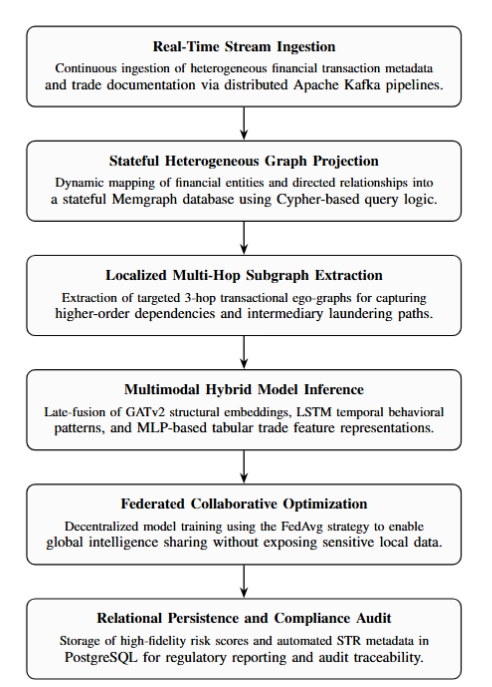
\includegraphics[
        width=\textwidth,
        height=0.8\textheight,
        keepaspectratio
    ]{./Figures/methodology.png}
}
{
    \fbox{
        \parbox[c][0.8\textheight][c]{0.95\textwidth}{
            \centering
            \Large Methodology Diagram Placeholder
        }
    }
}

\caption{Proposed Methodology for TBML Detection}
\label{fig:methodology}
\end{figure}


%========================================================
\section[Assumptions and Constraints of the Work]{\textbf{Assumptions and Constraints of the Work}}
%========================================================

\subsection*{Assumptions}

\begin{itemize}
    \item 
    
It is assumed that the financial transaction records, trade invoices, and customer in
formation utilized for the analysis process are structured, consistent, and preprocessed
in an appropriate manner.
    
    \item 
It is assumed that the involved financial institutions keep their transaction format and
standardized trade attributes similar enough for constructing graphs and analyzing sus
picious activity.
    
    \item 
It is assumed that the created financial datasets include enough normal and suspicious
patterns to learn hidden behavioral relationships between entities for detecting Trade-
Based Money Laundering activities.
    
    \item 
Heterogeneous graph representation is assumed to be capable of describing relations
between different objects including accounts, organizations, transactions, invoices, and
trade entities to detect suspicious financial behavior.
\end{itemize}

\subsection*{Constraints}

\begin{itemize}
    \item 
Evaluation using transactional data of participating financial institutions.
    
    \item 
The performance of the suggested method significantly relies on the quality and com
pleteness of financial datasets available for the training and testing purposes.
    
    \item 
Real-time graph construction and transactional analysis of the huge graph structure
may cause computational and memory overheads in fraud detection operations.
    
    \item 
The framework is verified mainly by means of experimental tests conducted under ac
ademic conditions.
\end{itemize}

\newpage
%========================================================
\section[Organization of the Report]{\textbf{Organization of the Report}}
%========================================================

This report is organized as follows.

\begin{itemize}

    \item 
In Chapter 2, theoretical foundations related to the Trade-Based Money Laundering
detection process, such as anti-money laundering schemes, heterogeneous graph rep
resentation, graph neural networks, and federated learning techniques are introduced.
    
    \item 
    
Chapter 3 demonstrates the Software Requirements Specification (SRS) of the pro
posed framework, which includes functional requirements, system constraints, software
and hardware requirements, and operating procedures.
    
    \item
The general structure of the proposed framework is provided in Chapter 4, where its
architecture, workflow, data flow scheme, and dashboard design are explained.
    
    \item 
Chapter 5 outlines the system design approach that involves constructing heteroge
neous graphs, performing fraud detection, designing STRs, and integrating com
pliance monitoring into the framework.
    
    \item 
Chapter 6 addresses the implementation steps taken during the creation of the pro
posed framework and include data preprocessing, graph construction, back end devel
opment, federated learning algorithm integration, and dashboard construction.
    
    \item 
 Chapter 7 assesses the processes used for testing and validating the proposed frame
work, including functional tests, fraud predictions analysis, dashboard evaluations, and
performance assessment.
    
    \item 
 In Chapter 8, the experimental outcomes and system performance are analyzed in terms
of fraud classification accuracy, scalability, and comprehensive system evaluation
    
    \item 
The ninth chapter provides an overall summary of the conclusions from the suggested work while also analyzing the existing limitations and future improvements of the framework.

\end{itemize}



